\documentclass{article}
\usepackage[latin1]{inputenc}
\usepackage{enumerate}
\usepackage{hyperref}
\usepackage{graphics}
\usepackage{graphicx}
\usepackage{caption}
\usepackage{subcaption}
\usepackage{tabularx}
\usepackage{amsmath}
\newcommand{\ket}[1]{\ensuremath{\left|#1\right\rangle}}
\newcommand{\bra}[1]{\ensuremath{\left\langle#1\right|}}
\newcommand{\braket}[2]{\ensuremath{\left\langle #1 \middle| #2 \right\rangle}}
\newcommand{\obar}[1]{\ensuremath{\overline{ #1 }}}
% enumerate is numbered \begin{enumerate}[(I)] is cap roman in parens
% itemize is bulleted \begin{itemize}
% subfigures:
% \begin{subfigure}[b]{0.5\textwidth} \includegraphics{asdf.jpg} \caption{} \label{subfig:asdf} \end{subfigure}
\hypersetup{colorlinks=true, urlcolor=blue, linkcolor=blue, citecolor=red}
\graphicspath{ {C:/Users/Evan/Desktop/} }
\title{Assignment 2: \\ Introduction to \emph{Mathematica}\\
\large \emph{Introduction to Data Analysis for Physics}}
\author{Evan Ott and Will Beason}
\date{Spring 2014}
\setcounter{secnumdepth}{0}
\usepackage[parfill]{parskip}
\begin{document}
\maketitle
\section{Submission Requirements}
Submit the assignment to \href{mailto:data.analysis.physics@gmail.com}{data.analysis.physics@gmail.com} by Wednesday at 5pm. Just submit the \emph{Mathematica}
document you create (typically a .nb file).

\section{Problem 1}
To start, let's make a simple set of data and use some of the stylistic options to make a graph exactly the way we want. Start with
\begin{verbatim}
data = Table[{i, Sin[.1 i]}, {i, 0, 100}]
\end{verbatim}
and create a plot that matches the one in Figure \ref{fig:listplot}. You may find the \texttt{Style} function useful (updated in reading - just above the Practice Problem for Simple Plots).
To create the plot, I had to use \texttt{PlotStyle, PlotRange, AxesLabel, PlotLabel}, and \texttt{AxesStyle}.

\begin{figure}
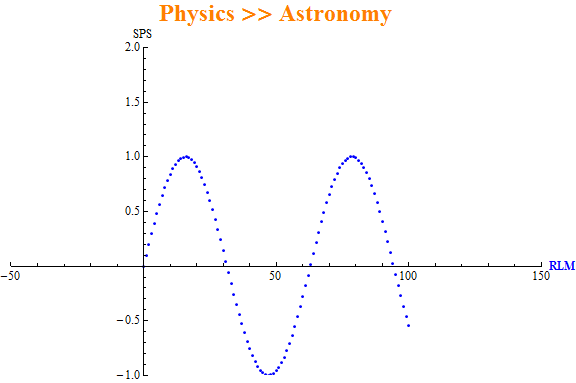
\includegraphics[scale=.6]{physics_astro.png}
\caption{Graph to imitate.}
\label{fig:listplot}
\end{figure}

\section{Problem 2}
Combinatorics are an important facet of probability, which occasionally shows up for physics problems in quantum mechanics / thermodynamics / etc. The \texttt{Binomial[n,m]} function
is the same as $$\left(\begin{array}{c}n\\m\end{array}\right)=\frac{n!}{m!(n-m)!}$$

To better explore matrix operations (and maybe learn some combinatorics), let\rq{}s create a 10x10 matrix with binomial coefficients:

$$A=\begin{pmatrix}
1 & 0 & 0 & 0 & 0 & \\
1 & 1 & 0 & 0 & 0 & \\
1 & 2 & 1 & 0 & 0 & \cdots\\
1 & 3 & 3 & 1 & 0 & \\
1 & 4 & 6 & 4 & 1 & \\
   &     &  \vdots & &    & \ddots
\end{pmatrix}$$

In other words, that $A_{r,c}=\begin{pmatrix}r-1 \\ c-1\end{pmatrix}$, where $r$ is the row (starting at 1) and $c$ is the column (starting at 1). Use the \texttt{Binomial}
function to create this matrix (will need to also use the \texttt{Table} command). In the problems below, use the \texttt{Total} command with sections of the matrix to compute the
following quantities. Each is left as a function of $k$, an integer corresponding to the total number of elements in the section. So, to check your work, just plug in different
values of $k$ to make sure the quantity you\rq{}re trying to compute with the matrix matches the mathematical result of sums of the binomial distribution.
(\textit{Note:} in \textit{Mathematica}, with the \texttt{Binomial[n,m]} function, if $m>n$, the function is just $0$)

\subsection{a}
$$\sum_{i=0}^k \begin{pmatrix}i\\1\end{pmatrix}=\frac{k(k+1)}{2}$$

\subsection{b}
$$\sum_{i=0}^k \begin{pmatrix}k \\ i\end{pmatrix}=2^k$$

\section{Problem 3}
With the data below, find a way to plot the relationship between the second grade (taken at the end of the semester for this fictional class) and the first grade multiplied by attendance
(scale attendance from a percent to a fraction while you're at it). For clarity, go ahead and make the points \texttt{Medium} in size, and label the graph appropriately.

\begin{verbatim}
class = {{"Name", "Grade 1", "Grade 2", "Attendance"},
   {"Michael", 95, 93, 20},
   {"George", 95, 87, 90},
   {"Oscar", 50, 78, 60},
   {"Lucille", 100, 0, 10},
   {"Lindsay", 40, 40, 40},
   {"Steve", 0, 0, 100},
   {"Barry", 50, 50, 50},
   {"Ron", 100, 100, 57},
   {"Rita", 10, 20, 97},
   {"Sally", 100, 100, 100},
   {"Maggie", 77, 76, 75}};
\end{verbatim}



\end{document}